% Versões de slide dos Quadros 3 e 4 e da Figura 6 do TG (13/11/2026, pedido do
% autor). NÃO é parte do TG. As versões completas estão no tg/ (Quadro 3 no Cap. II,
% Quadro 4 no Cap. III). PNG de cada uma gerado pelo Makefile, para o PowerPoint.
\documentclass[11pt,a4paper]{article}
\usepackage[T1]{fontenc}
\usepackage[brazilian]{babel}
\usepackage{mathptmx}
\usepackage[a4paper,margin=2.4cm]{geometry}
\usepackage{graphicx}
\usepackage[font=small,labelfont=bf]{caption}
\usepackage[most]{tcolorbox}
\usepackage[hidelinks]{hyperref}
\setlength{\parskip}{0.45em}
\setlength{\parindent}{0pt}
\definecolor{cmod}{RGB}{0,90,181}
\newtcolorbox{ideia}[1][]{colback=cmod!5, colframe=cmod!70, fonttitle=\bfseries, title={#1}, arc=2pt, boxrule=0.6pt}

\title{Quadros para os slides da defesa\\[2pt]\large versões simples dos Quadros 3 e 4}
\author{Material de apoio, fora do TG}
\date{13 de novembro de 2026}

\begin{document}
\maketitle

O texto do TG ficou com as versões completas: o Quadro~3 (configurações testadas)
separado em parte comum e parte própria de cada forma de uso do GARCH, e o
Quadro~4 (configuração de cada robô escolhido) com todos os parâmetros, inclusive o
ARIMA sem GARCH. Para os slides, as duas tabelas abaixo dizem o mesmo com menos
coisa, em letra grande e sem serifa. Os arquivos \texttt{slide-quadro3.png},
\texttt{slide-quadro4.png} e \texttt{slide-integracao.png} desta pasta são para
colar no PowerPoint.

\section{Configurações testadas (Quadro 3)}

\begin{center}
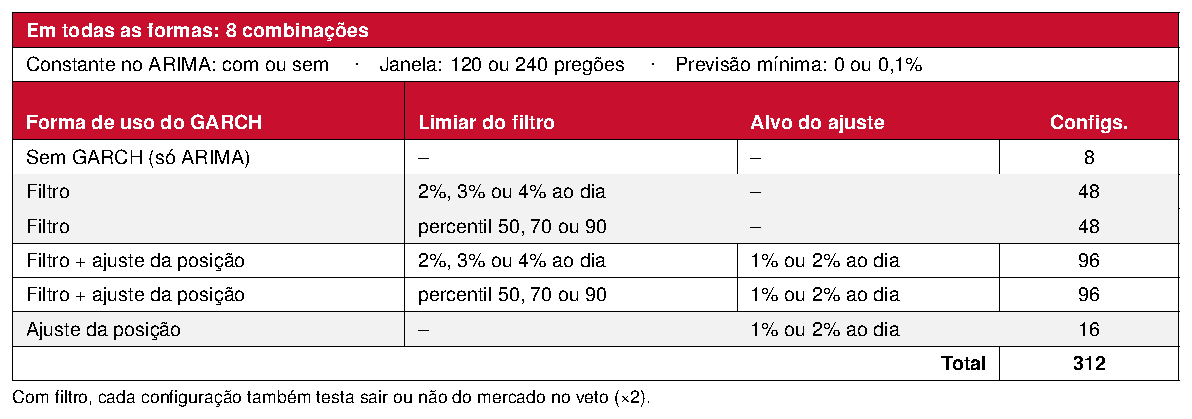
\includegraphics[width=\linewidth]{slide-quadro3.pdf}
\end{center}

Igual ao Quadro~3 do TG, só que a opção de sair ou não do mercado no veto saiu da
tabela e virou a linha de baixo, e as contas ($8 \times 3 \times 2$...) ficaram
só no TG. Na fala: ``tudo começa com 8 combinações do ARIMA; cada forma de usar o
GARCH multiplica essas 8 pelos valores dela; ao todo, 312''.

\section{O que cada robô escolheu (Quadro 4)}

\begin{center}
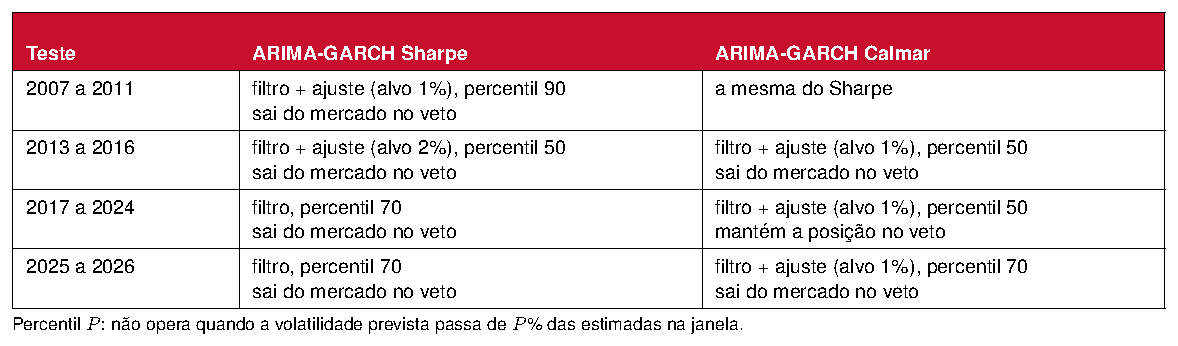
\includegraphics[width=\linewidth]{slide-quadro4.pdf}
\end{center}

Só a forma de uso do GARCH, que é o assunto do trabalho. Ficaram de fora, e estão
no Quadro~4 do TG: a janela, a constante e a previsão mínima do ARIMA, o índice que
definiu a escolha e a linha do ARIMA sem GARCH. ``Sai do mercado no veto'' é o que
o TG chama de ``encerra a posição no veto''.

\begin{ideia}[O que dá para dizer olhando este quadro]
Todos os robôs escolhidos usam o filtro, e todos com limiar por percentil, nenhum
com limiar fixo. Em quase todos, o veto também tira o robô do mercado. A exceção é
o ARIMA-GARCH Calmar de 2017 a 2024, que mantém a posição durante o veto, e o TG
liga isso ao resultado dele naquele período.
\end{ideia}

\section{Integração entre ARIMA e GARCH (Figura 6)}

A Figura~6 do TG foi refeita como o ciclo de um pregão, sem fórmula, e já serve
para slide do jeito que está (\texttt{slide-integracao.png} é cópia dela). Se o
veto acontece, o pregão termina sem ordem e o ciclo recomeça no pregão seguinte.

\begin{center}
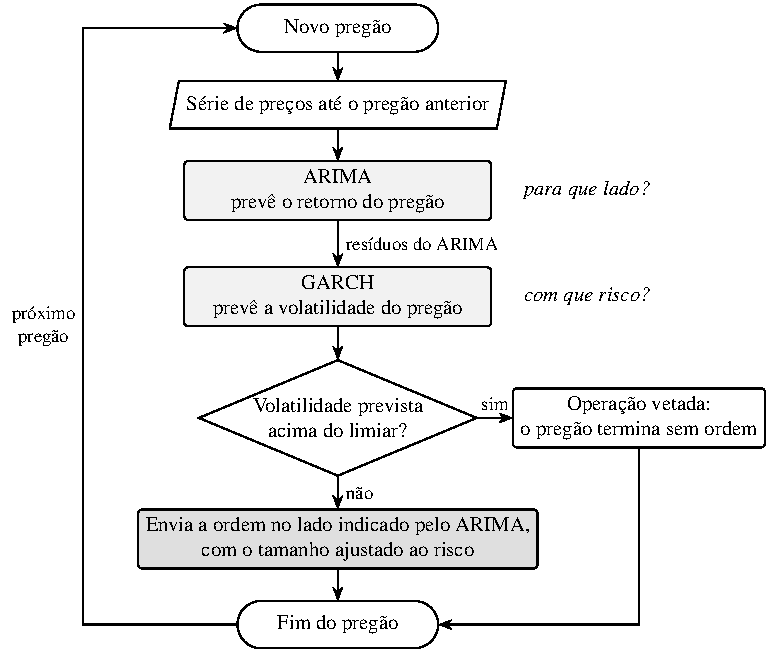
\includegraphics[width=0.75\linewidth]{slide-integracao.pdf}
\end{center}

\section{Procedência}

As linhas do Quadro~4 (aqui e no TG) foram geradas por \texttt{awk} a partir de
\texttt{dados/resultados/refeito\_2026-10-05/escolhas/r3\_C1..C3.txt} e
\texttt{r6\_C4.txt}, sem digitar valor. Os valores do Quadro~3 são os das grades
\texttt{grades/r3\_*.txt} da mesma pasta.

\end{document}
